\begin{usecase}{Connect Calendar}
  \ucbasicinfo{Medium}{Regular}
  \ucshortdescription{This UC allows the user to add Jadwal's Baikal calendar credentials using a .mobileconfig profile to their iOS device calendar accounts.}
  \uctrigger{This UC is triggered when the user wants clicks ``Easy Setup'' in the mobile app.}
  \ucactors{User}{iOS Settings}
  \ucpreconditions{User must be logged in}
  \ucrelationships{N/A}{N/A}{N/A}
  \ucinputsoutputs{
    \begin{itemize}
      \item \textbf{Magic Token with type CalDav} (Source: System)
      \item \textbf{.mobileconfig profile} (Source: System)
    \end{itemize}
  }{
    \begin{itemize}
      \item \textbf{Calendar configuration status} (Destination: iOS Settings)
    \end{itemize}
  }
  \ucmainflow{
    \begin{enumerate}
      \item The user taps "Easy Setup" in the app.
            \ucinfo{The app calls the backend to get a Magic Token of type CalDAV.}
      \item The app prompts the user to download the file from the backend endpoint.
            \ucinfo{The Magic Token is used to authenticate the user and get his credentials and give him his unique file to download.}
      \item The user approves the profile installation.
            \ucinfo{iOS configures the CalDAV account with our Baikal server automatically.}
      \item The app shows the user a success page when he goes back to it.
            \ucinfo{Success is shown only after confirming the calendar configuration is complete.}
    \end{enumerate}
  }
  \ucalternateflows{
    \begin{enumerate}
      \item If the user denies profile installation:
            \begin{itemize}
              \item The app shows an error page with "Setup cancelled - Try again later"
              \item The user can retry the setup process later
            \end{itemize}
      \item If the calendar configuration fails:
            \begin{itemize}
              \item The app shows an error page with "Calendar setup failed"
              \item The user may need to contact support or retry the process
            \end{itemize}
    \end{enumerate}
  }

  \ucconclusion{The UC ends when either the calendar is successfully configured or an error page is shown to the user.}
  \ucpostconditions{Either the user's iOS device is configured to sync with our Baikal calendar server, or the user is informed of the failure with appropriate guidance.}
  \ucspecialrequirements{The system must generate secure, user-specific .mobileconfig profiles.}
\end{usecase}

\begin{figure}[!h]
  \centering
  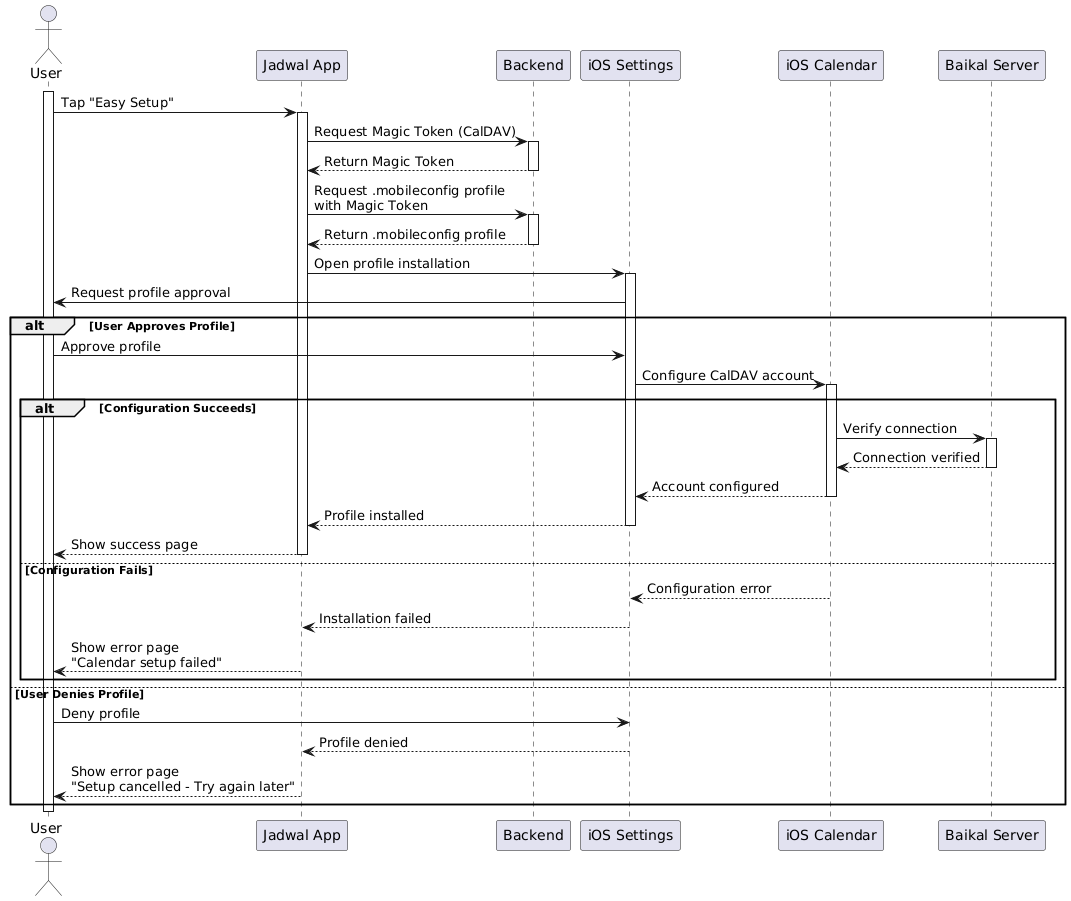
\includegraphics[width=\textwidth]{images/docs/diagrams/sequence-diagrams/all-sequence-diagrams/Connect Calendar.png}
  \caption{Connect Calendar Sequence Diagram}
  \label{fig:seq/connect-calendar}
\end{figure}

The ``Connect Calendar Sequence Diagram'', shown in \textbf{Figure~\ref{fig:seq/connect-calendar}}, illustrates the streamlined process of connecting an iOS device to Jadwal's Baikal calendar server. The sequence begins when the user taps ``Easy Setup'' in the app.

The process follows a secure flow where the app first requests a Magic Token of type CalDAV from the backend. Using this token, the app then requests a user-specific \textit{.mobileconfig} profile that contains the pre-configured CalDAV credentials. When the user downloads this profile, iOS Settings takes over to handle the secure installation process.

The diagram illustrates the following possible paths:
\begin{enumerate}
  \item \textbf{Success Path:} The user approves the profile installation in iOS Settings, which then automatically configures the CalDAV account. Upon returning to the app, the user is shown a success page after the system confirms the calendar configuration is complete.
  \item \textbf{User Denial Path:} If the user denies the profile installation, they return to the app which displays "Setup cancelled - Try again later", allowing them to retry the process at their convenience.
  \item \textbf{Configuration Failure Path:} If the profile installation is approved but the calendar configuration fails, the app shows a "Calendar setup failed" message, prompting the user to either contact support or retry the process.
\end{enumerate}

This implementation leverages iOS's native configuration profile system to ensure a secure and user-friendly setup process. The use of Magic Tokens and encrypted \textit{.mobileconfig} profiles during transit guarantees that calendar credentials are transmitted and stored securely on the user's device. The clear error handling paths ensure users receive appropriate guidance when issues occur during any stage of the setup process.